\chapter{Lezione 24}
\label{chap:lezione_24}

\begin{flushright}
\textit{Data: 22/12/2025}
\end{flushright}


\section{Rinormalizzazione nello Spazio Reale}


Nelle lezioni precedenti l'analisi del Gruppo di Rinormalizzazione (RG) è stata condotta prevalentemente nello \textit{spazio dei momenti}, effettuando il rescaling dei momenti. 
In questa sezione adottiamo un approccio complementare, lavorando direttamente nello \textbf{spazio reale}. 

L'intuizione fisica alla base di questo metodo risiede nel comportamento della lunghezza di correlazione $\xi$ in prossimità del punto critico $T_c$:
\begin{equation}
    \xi \to \infty \quad \text{per} \quad T \to T_c
\end{equation}
Dato che le fluttuazioni diventano correlate su distanze macroscopiche, i dettagli microscopici a scala di reticolo perdono rilevanza. È quindi possibile raggruppare i gradi di libertà (spin) in "blocchi" o cluster, definendo delle variabili efficaci che descrivono il comportamento collettivo del sistema. Questo processo di \textit{coarse graining} permette di costruire una teoria efficace a scale di lunghezza maggiori, eliminando progressivamente le fluttuazioni a corto raggio.

% -------------------------------------------------------------------
\subsection{Relazioni di Scaling}


L'ipotesi di scaling impone vincoli precisi sugli esponenti critici. Analizziamo le conseguenze sulla funzione di correlazione a due punti, che vicino alla criticità assume la forma:
\begin{equation}
    G(r) \sim \frac{1}{r^{d-2+\eta}} f\left(\frac{r}{\xi}\right)
\end{equation}
dove $d$ è la dimensione spaziale e $\eta$ l'esponente anomalo. Definita la temperatura ridotta $\theta = \frac{T - T_c}{T_c}$, sappiamo che la  lunghezza di correlazione diverge come $\xi \sim |\theta|^{-\nu}$.

\noindent Il comportamento asintotico di $G(r)$ si divide in tre regimi fondamentali:
\begin{enumerate}
    \item \textbf{Regime Critico ($r \ll \xi$):}  Il sistema si comporta come se fosse esattamente al punto critico ($T=T_c$). La correlazione decade a potenza:
    \begin{equation}
        G(r) \sim \frac{1}{r^{d-2+\eta}}
    \end{equation}
    Non c'è una scala intrinseca (invarianza di scala).
    
    \item \textbf{Regime di Transizione ($r \sim \xi$):} Si passa dal comportamento a potenza a quello esponenziale.
    
    \item \textbf{Regime Disordinato ($r \gg \xi$):} Le correlazioni decadono esponenzialmente:
    \begin{equation}
        G(r) \sim e^{-r/\xi}
    \end{equation}
    La lunghezza di correlazione funge da cutoff per le fluttuazioni critiche.
\end{enumerate}

\subsection{Legge di Hyperscaling (Relazione di Josephson)}
L'ipotesi di \textbf{Hyperscaling} collega la termodinamica alla geometria delle fluttuazioni, assumendo che l'energia libera singolare per unità di volume scali come l'inverso del volume di correlazione:
\begin{equation}
    F_{sing} \sim \xi^{-d} \sim |\theta|^{d\nu}
\end{equation}
Poiché il calore specifico è legato alla derivata seconda dell'energia libera:

\begin{equation}
   C_V \sim \frac{\partial^2 F }{ \partial \theta^2 } \sim |\theta|^{-\alpha}
\end{equation}

integrando due volte si ottiene $F_{sing} \sim |\theta|^{2-\alpha}$. Il confronto tra le due stime conduce alla relazione:

\begin{tcolorbox}[colback=yellow!25, colframe=yellow!75!orange, coltitle=black, title=\textbf{Relazione di Josephson}]
\begin{equation}
    2 - \alpha = d \nu
    \label{eq:hyperscaling}
\end{equation}
\end{tcolorbox}

\subsection{Scaling della Suscettibilità (Legge di Fisher)}
Sfruttando il teorema fluttuazione-dissipazione, possiamo esprimere la suscettibilità magnetica $\chi$ come l'integrale della funzione di correlazione su tutto il volume:
\begin{equation}
    \chi \sim \int d^d r \, G(r) \approx \int d^d r \, \frac{1}{r^{d-2+\eta}} f\left(\frac{r}{\xi}\right)
\end{equation}
Operando il cambio di variabile $x = r/\xi$ (da cui $d^d r = \xi^d d^d x$), l'integrale diventa:
\begin{equation}
    \chi \sim \xi^d \xi^{-(d-2+\eta)} \int d^d x \, \frac{f(x)}{x^{d-2+\eta}} 
\end{equation}

\noindent L'integrale adimensionale converge a una costante (assumendo che $f (x)$ decada abbastanza
rapidamente per $x \gg 1$). Quindi la dipendenza critica è tutta nel pre-fattore:
\begin{equation}
    \chi \sim \xi^{d - (d-2+\eta)} = \xi^{2-\eta}
\end{equation}

\noindent Ricordando che la lunghezza di correlazione diverge come $\xi \sim |\theta|^{-\nu}$ e che la suscettibilità diverge per definizione come $\chi \sim |\theta|^{-\gamma}$, otteniamo la \textbf{legge di Fisher}:

\begin{tcolorbox}[colback=yellow!25, colframe=yellow!75!orange,  coltitle=black, title=\textbf{Legge di Fisher}]
\begin{equation}
    \gamma = \nu(2-\eta)
\end{equation}
\end{tcolorbox}

\noindent Questa equazione è estremamente importante perché collega una quantità termodinamica ($\gamma$) con esponenti legati alla struttura spaziale delle correlazioni ($\nu$ e $\eta$).

\noindent Riassumendo, le relazioni di scaling permettono di ridurre il numero di esponenti indipendenti. Le quattro identità principali sono:

\begin{tcolorbox}[colback=colorA!10, colframe=colorA, coltitle=white, title=\textbf{Relazioni tra Esponenti Critici}]
\begin{align}
   \alpha &= 2-\nu d & \beta &= \frac{\nu(d-2+\eta)}{2} \\
   \gamma &= \nu(2-\eta) & \delta &= \frac{(d+2-\eta)}{d+2+\eta}
\end{align}
\end{tcolorbox}

Con $\alpha$ l'esponente critico del calore specifico, $\beta$ l'esponente critico della magnetizzazione, $\gamma$ l'esponente critico della suscettibilità, $\delta$ l'esponente critico della funzione di Green a $\theta$=0 e $\nu$ l'esponente critico della legge di correlazione a $T_c$

% -------------------------------------------------------------------
\section{Metodo del Block Spin di Kadanoff}
\label{sec:blockspin}

Il metodo del \textbf{Block Spin} (introdotto da Kadanoff) formalizza il RG nello spazio reale. Dato un reticolo di passo $a$, la procedura si articola in passi iterativi:
\begin{enumerate}
    \item \textbf{Raggruppamento:} Si partiziona il reticolo in blocchi di lato $\lambda a$ ($\lambda > 1$).
    \item \textbf{Definizione Variabile Efficace:} Ad ogni blocco $B_I$ si associa uno spin $\sigma'_I$ che rappresenta lo stato medio del blocco, determinato ad esempio dalla regola della maggioranza:
    \begin{equation}
        \sigma'_I = \text{sgn}\left(\sum_{i \in B_I} \sigma_i\right)
    \end{equation}
    \item \textbf{Decimazione:} Si costruisce la funzione di partizione sommando sui gradi di libertà interni, vincolando il valore dello spin di blocco. Formalmente:
    \begin{equation}
        Z = \sum_{\{\sigma\}} e^{-H(\sigma)} = \sum_{\{\sigma'\}} e^{-H'(\sigma')}
    \end{equation}
    L'azione efficace $H'$ è definita da:
    \begin{equation}
        e^{-H'(\sigma')} = \sum_{\{\sigma\}} \left( \prod_I \delta\left(\sigma'_I - f(\{\sigma\}_{B_I})\right) \right) e^{-H(\sigma)}
    \end{equation}
    \item \textbf{Rescaling:} Si riportano le lunghezze alla scala originale tramite la trasformazione $x' = x/\lambda$.
\end{enumerate}

Il fulcro del metodo è determinare la mappa di rinormalizzazione dei parametri dell'Hamiltoniana, $K' = \mathcal{R}(K)$ (dove $K = \beta J$), i cui punti fissi identificano le transizioni di fase.

% -------------------------------------------------------------------
\section{Decimazione del Modello di Ising 1D}
\label{sec:decimazione}

Il modello di Ising unidimensionale rappresenta uno dei rari casi risolubili esattamente tramite la tecnica della \textbf{decimazione}.
Consideriamo una catena chiusa di $N$ spin con condizioni al contorno periodiche ($\sigma_{N+1} = \sigma_1$).  L'Hamiltoniana ridotta (assumendo campo esterno $h=0$) è:
\begin{equation}
    -\beta H = K \sum_{i=1}^N \sigma_i \sigma_{i+1}
\end{equation}
La funzione di partizione è:
\begin{equation}
    \mathcal{Z}_N = \sum_{\{\sigma\}} e^{K \sum_i \sigma_i \sigma_{i+1}} = \sum_{\{\sigma\}} \prod_{i=1}^N T(\sigma_i, \sigma_{i+1})
\end{equation}
dove $T(\sigma_i, \sigma_{i+1}) = e^{K \sigma_i \sigma_{i+1}}$ è la matrice di trasferimento.

\subsubsection{Procedura di Decimazione}
Eseguiamo la somma parziale sugli spin situati nei siti pari (es. $\sigma_2$), lasciando inalterati i siti dispari. Isoliamo i termini che coinvolgono $\sigma_2$:
\begin{equation}
    \sum_{\sigma_2 = \pm 1} e^{K \sigma_1 \sigma_2 + K \sigma_2 \sigma_3} = \sum_{\sigma_2 = \pm 1} e^{K \sigma_2 (\sigma_1 + \sigma_3)}
\end{equation}
Valutando esplicitamente la somma per i due stati possibili di $\sigma_2$:
\begin{itemize}
    \item $\sigma_2 = +1 \implies e^{K(\sigma_1 + \sigma_3)}$
    \item $\sigma_2 = -1 \implies e^{-K(\sigma_1 + \sigma_3)}$
\end{itemize}
si ottiene il risultato:
\begin{equation}
    2 \cosh(K(\sigma_1 + \sigma_3))
\end{equation}

\hfill

\begin{figure}[h]
    \centering
    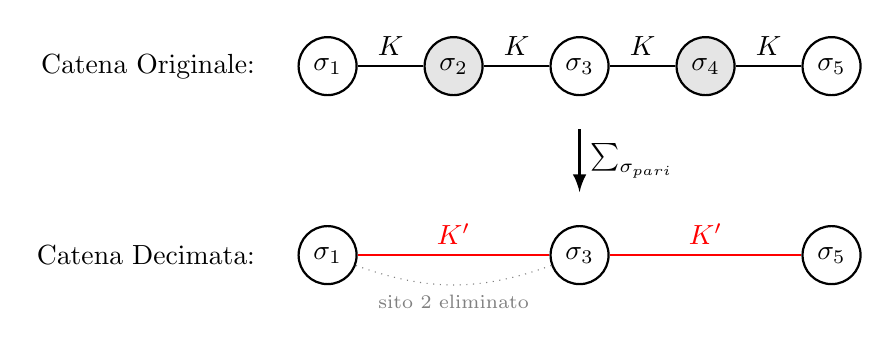
\begin{tikzpicture}[node distance=1.5cm, scale=0.8]
        % CATENA ORIGINALE
        \node[circle, draw, thick, fill=white] (s1) at (0,0) {$\sigma_1$};
        \node[circle, draw, thick, fill=gray!20] (s2) at (2,0) {$\sigma_2$};
        \node[circle, draw, thick, fill=white] (s3) at (4,0) {$\sigma_3$};
        \node[circle, draw, thick, fill=gray!20] (s4) at (6,0) {$\sigma_4$};
        \node[circle, draw, thick, fill=white] (s5) at (8,0) {$\sigma_5$};
        \draw[thick] (s1) -- (s2) node[midway, above] {$K$};
        \draw[thick] (s2) -- (s3) node[midway, above] {$K$};
        \draw[thick] (s3) -- (s4) node[midway, above] {$K$};
        \draw[thick] (s4) -- (s5) node[midway, above] {$K$};
        \node[anchor=east] at (-1,0) {Catena Originale:};
        
        \draw[->, very thick, >=latex] (4, -1) -- (4, -2) node[midway, right] {$\sum_{\sigma_{pari}}$};

        % CATENA DECIMATA
        \begin{scope}[yshift=-3cm]
            \node[circle, draw, thick, fill=white] (t1) at (0,0) {$\sigma_1$};
            \node[circle, draw, thick, fill=white] (t3) at (4,0) {$\sigma_3$};
            \node[circle, draw, thick, fill=white] (t5) at (8,0) {$\sigma_5$};
            \draw[thick, red] (t1) -- (t3) node[midway, above] {$K'$};
            \draw[thick, red] (t3) -- (t5) node[midway, above] {$K'$};
            \draw[dotted, gray] (t1) to[bend right=20] node[midway, below] {\scriptsize sito 2 eliminato} (t3);
            \node[anchor=east] at (-1,0) {Catena Decimata:};
        \end{scope}
    \end{tikzpicture}
    \caption{Rappresentazione grafica della decimazione: eliminazione dei siti pari e rinormalizzazione dell'accoppiamento tra i siti rimanenti.}
    \label{fig:decimazione}
\end{figure}

\hfill

Il passo successivo consiste nel riscrivere questo risultato nella forma di un'interazione efficace tra i primi vicini rimasti ($\sigma_1, \sigma_3$), introducendo un nuovo accoppiamento $K'$ e una costante $C$:
\begin{equation}
    C e^{K' \sigma_1 \sigma_3} = 2 \cosh(K(\sigma_1 + \sigma_3))
\end{equation}
Uguagliamo le due espressioni per le possibili configurazioni di $\sigma_1$ e $\sigma_3$:
\begin{enumerate}
    \item \textbf{Spin paralleli} ($\sigma_1 = \sigma_3 \implies \sigma_1 + \sigma_3 = \pm 2$):
    \begin{equation}
        2 \cosh(2K) = C e^{K'}
    \end{equation}
    \item \textbf{Spin antiparalleli} ($\sigma_1 = -\sigma_3 \implies \sigma_1 + \sigma_3 = 0$):
    \begin{equation}
        2 \cosh(0) = 2 = C e^{-K'}
    \end{equation}
\end{enumerate}



Risolvendo il sistema per $C$ e $K'$ (moltiplicando e dividendo le equazioni membro a membro), otteniamo la costante di normalizzazione $C = 2 \sqrt{\cosh(2K)}$ e, soprattutto, la legge di trasformazione per l'accoppiamento:

\begin{tcolorbox}[colback=yellow!25, colframe=yellow!75!orange,  coltitle=black,  title=\textbf{Relazione di ricorrenza del Gruppo di Rinormalizzazione}]
\begin{equation}
    K' = \frac{1}{2} \ln[\cosh(2K)]
\end{equation}
\end{tcolorbox}


\subsubsection{Analisi del Flusso}
Possiamo introdurre la variabile $x = \tanh K$ (o $x = e^{-2K}$). Spesso è comodo usare $v = \tanh K$.
Ricordando che $\cosh(2K) = \frac{1 + \tanh^2 K}{1 - \tanh^2 K}$ o usando le identità iperboliche, possiamo vedere che la trasformazione spinge l'accoppiamento verso valori specifici.

Analizziamo i punti fissi $K^* = f(K^*)$:
\begin{itemize}
    \item \textbf{$K^* = \infty$ ($T=0$):} Se $K \to \infty$, $\cosh(2K) \approx e^{2K}/2$.
    $$ K' \approx \frac{1}{2} \ln(e^{2K}/2) = K - \frac{1}{2}\ln 2 $$
    Questo è un punto fisso instabile (tutto il flusso a bassa temperatura tende qui, ma nel limite termodinamico 1D non c'è ordine a $T>0$).
    
    \item \textbf{$K^* = 0$ ($T=\infty$):} Se $K \to 0$, $\cosh(2K) \approx 1$.
    $$ K' \approx \frac{1}{2} \ln(1) = 0 $$
    Questo è il punto fisso stabile che attrae ogni $K$ finito. Ogni temperatura finita $T > 0$ fluisce verso $T = \infty$ (sistema disordinato).
\end{itemize}

% FIGURA FLUSSO RG INTEGRATA
\begin{figure}[h]
    \centering
    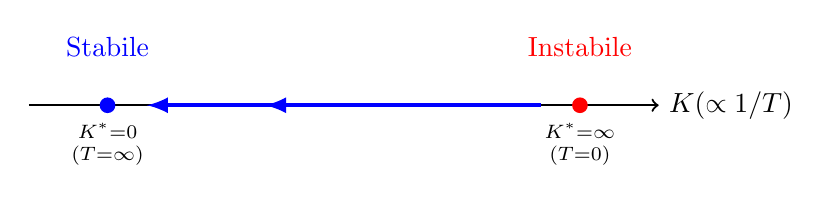
\begin{tikzpicture}[scale=1]
        % Asse K
        \draw[->, thick] (-1,0) -- (7,0) node[right] {$K (\propto 1/T)$};
        
        % Punti fissi
        \node[circle, fill=blue, inner sep=2pt, label=below:{$K^*=0 \atop (T=\infty)$}] (k0) at (0,0) {};
        \node[circle, fill=red, inner sep=2pt, label=below:{$K^*=\infty \atop (T=0)$}] (kinf) at (6,0) {};
        
        % Frecce di flusso
        \draw[->, ultra thick, blue, >=latex] (5.5, 0) -- (0.5, 0);
        \draw[->, ultra thick, blue, >=latex] (3, 0) -- (2, 0);
        
        % Etichette di stabilità
        \node[above=0.5cm, blue] at (0,0) {Stabile};
        \node[above=0.5cm, red] at (6,0) {Instabile};
        
        
    \end{tikzpicture}
    \caption{Diagramma del flusso di rinormalizzazione per il modello di Ising 1D. Ogni accoppiamento finito $K$ fluisce verso il punto fisso stabile a $K=0$ (temperatura infinita), indicando l'assenza di una fase ordinata a temperatura finita.}
    \label{fig:rg_flow}
\end{figure}

La decimazione in 1D mostra che non c'è transizione di fase a temperatura finita, poiché l'unico punto fisso critico (instabile) è a $T=0$ ($K=\infty$). Qualsiasi $K < \infty$ viene rinormalizzato a $K=0$ iterando la trasformazione.
